\hypertarget{dane_8cpp}{\section{dane.\-cpp File Reference}
\label{dane_8cpp}\index{dane.\-cpp@{dane.\-cpp}}
}


Plik z definicjami metod dla klasy dane.  


{\ttfamily \#include $<$iostream$>$}\\*
{\ttfamily \#include $<$fstream$>$}\\*
{\ttfamily \#include $<$cmath$>$}\\*
{\ttfamily \#include $<$ctime$>$}\\*
{\ttfamily \#include \char`\"{}dane.\-h\char`\"{}}\\*
Include dependency graph for dane.\-cpp\-:\nopagebreak
\begin{figure}[H]
\begin{center}
\leavevmode
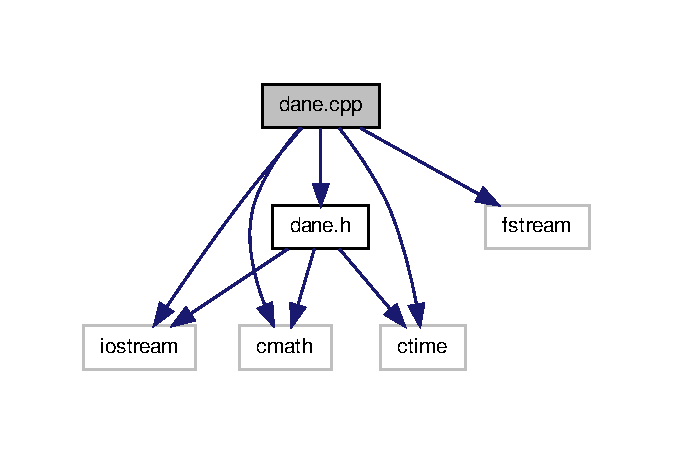
\includegraphics[width=323pt]{dane_8cpp__incl}
\end{center}
\end{figure}


\subsection{Detailed Description}
Plik zawiera definicje metod klasy dane tj. wyliczania wartosci odchylenia standardowego oraz zapisywania danych do pliku formatu csv. Ponadto zawiera definicje konstruktora parametrycznego w ktorym alokowana jest tablica do ktorej beda wpisywane czasy poszczegolnych powtorzen. 

Definition in file \hyperlink{dane_8cpp_source}{dane.\-cpp}.

